\documentclass[10pt]{article}
\usepackage{kennyworkman}

\newcommand\restr[2]{{% we make the whole thing an ordinary symbol
  \left.\kern-\nulldelimiterspace % automatically resize the bar with \right
  #1 % the function
  \vphantom{\big|} % pretend it's a little taller at normal size
  \right|_{#2} % this is the delimiter
}}

\title{Hatcher: Algebraic Topology}
\author{Kenny Workman}
\date{\today}

\begin{document}

\maketitle

\section{The Fundamental Group}

\subsection{Intuition}

\textbf{The Borromean rings} are three linked circles where any two circles without a third are unlinked. It is a nice object that elucidates the difference between abelian and nonabelian fundamental groups.

Label the three rings $A$, $B$, and $C$. Consider $C$ as an element of $\R^3 \setminus A \cup B$. $C$ can be represented as $aba^{-1}b^{-1}$, where $a$ and $a^{-1}$ are forward and reverse oriented paths around $A$ (and $B$). This element is not trivial, so the free group generated by $a$ and $b$ is not abelian.

Modify the ring so that $A$ and $B$ are linked. The same $C = aba^{-1}b^{-1}$ is now trivial. It is easiest to see this visually. Refer to the picture in Hatcher and slide the first loop $a$ all the way around $A$ until it is hanging over the circle. This loop is clearly contractible.

From this, we conclude there are two ways to tell if two circles are linked:

\begin{itemize}
	\item{Show that one of the circles is an element of the fundamental group of the complement of the other circle. (Simple example of loop wrapping around a circle.)}
	\item{Show the fundamental group of the complement of both of the circles is the abelian. (As in the Borromean ring example.)}
\end{itemize}

\subsection{Basic Constructions}

\begin{definition}[Path]
A path in the space $X$ is a continuous map $f: I \to X$ where $I$ is the unit interval $[0, 1]$.
\end{definition}

\begin{definition}[Homotopy of paths]
A continuous family of maps represented by the continuous map $f: I \times I \to X$ 
\end{definition}

\begin{example}[Linear homotopy]
Consider two paths $f, g$ that share endpoints ($f(0) = g(0) = x_0$ and $f(1) =
g(1) = x_1$). Any such paths are always homotopic by the homotopy 
\[
h_t(s) = (1-t)f(s) + (t)g(s).
\]

% TODO: show continuity with vector argument

\end{example}


\begin{proposition}[homotopy of paths with fixed endpoints is an equivalence relation]
\end{proposition}

\begin{definition}[The product of paths]

	For paths $f, g$ where $f(1) = g(0)$, we can define the product $h = f \cdot g$ as

\[ h(s) = \begin{cases} 
      f(2s) & 0 \leq s \leq 0.5 \\
      g(2s-1) & 0.5 \leq s \leq 1
   \end{cases}
\]

\end{definition}


\begin{proposition}[The fundamental group is in fact a group]
	$\pi_1(X, x_0)$ with respect to the operator $[f]\cdot[g] = [f\cdot g]$ is a group.
\end{proposition}

\begin{definition}[Reparamterization of a path]
	We can precompose any path $f$ with $\phi: I \to I$ such that $f\phi \simeq f$. $f\phi$ is then the reparameterization of $f$.
\end{definition}

\begin{proof}
	To see our operator is well-defined, $[f\cdot g]$ depends only on $[f]$ and $[g]$. In other words, a homotopy exists between paths in $[f\cdot g]$ if and only if it is the composite of homotopies between paths in $[f]$ and $[g]$.

	First, we verify associativity of the operator. Consider $(f \cdot g) \cdot h$. This product composes the composition of $f$ and $g$ with $h$. Visually, $h$ is the first half and $g$ and $f$ occupy the last quarters of the product path. We can construct a piecewise function to change the proportions of these components - "shrink" $h$, keep $g$ the same and "expand" $f$. $[(f \cdot g) \cdot h]\phi \simeq f \cdot (g \cdot h)$ gives us the desired equivalence.

	Second, we check the identity property of the constant map $c$. $f$ can be reparameterized by the piecewise function that speeds it up for the first half of $I$ and holds it constant at $f(1)$ for the second half where $f\phi \simeq f \cdot c$.

	Third, we verify the existence of an inverse for each $[f]$. Define $[\bar{f}]$ where $\bar{f}(s) = f(1-s)$. Then $f\cdot\bar{f}$ is homotopic to the constant path. To see this construct $h_t = f_tg_t$ where $f_t = f$ on $[0, t]$ and $f_t = f(t)$ on $[1-t, 1]$ and $g_t$ is the inverse of this function. As $t$ approaches $1$, $h_t$ has a larger constant region in its image starting from the middle and growing to the endpoints until $h_1(s) = f(0) = g(1)$ is our constant map at timepoint 1.

\end{proof}

\begin{proposition}[The fundamental group is independent of the choice of basepoint up to isomorphism]
	If $f$ is a loop with basepoint $x_1$ and $h$ is a path from $x_0$ to $x_1$. The map $\beta_h: \pi_1(X, x_0) \to \pi_1(X, x_1)$ defined as $\beta_h([f]) = [h \cdot f \cdot \hat{h}]$ is an isomorphism.
\end{proposition}
\begin{proof}
	$\beta_h$ is well-defined. To see this, if $[f] = [f']$ implies that $f$ and $f'$ are homotopic, so certainly $h \cdot f \cdot \bar{h}$ and $h \cdot f' \cdot \bar{h}$ are homotopic and $\beta_h([f]) = \beta([f'])$.
	$\beta_h$ is a homomorphism. $\beta_h([f \cdot g]) = [h \cdot f \cdot g \cdot \bar{h}] = [h \cdot f \cdot \cdot h \cdot \bar{h} \cdot g \cdot \bar{h}] = [h \cdot f \cdot \cdot h] \cdot [\bar{h} \cdot g \cdot \bar{h}] = \beta_h([f]) \cdot = \beta_h([g])$. 
	$\beta_h$ is an isomorphism.

\end{proof}

\begin{definition}
	A space is \textbf{simply connected} if it is path connected and has a trivial fundamental group.
\end{definition}


\begin{theorem}[$\Z \cong \pi_1(S^1)$]

The map $\phi$ sending the integer $n$ to the homotopy class of the loop $\omega_n(x) = (cos2\pi nx, sin2\pi nx)$ on $S^1$ with basepoint $(1, 0)$ is an isomorphism.

\end{theorem}

\begin{proof}

Observe that each loop $\omega_n$ can be expressed as the composition
$p\tilde{\omega}_n$, where $p(s) = (cos2\pi s, sin2\pi s)$ and
$\tilde{\omega}_n(s) = ns$ is the path in $\R$ from $0$ to $n$.
$\tilde{\omega}_n$ is called the \textbf{lift} of $\omega_n$.

We define the image of $n \in Z$ under $\phi$ as the homotopy class represented
by $pf_n$ where $f_n$ is any path in $\R$ from $0$ to $n$. Since any such $f_n$
shares endpoints with $\tilde{\omega}_n$, the paths are homotopic, and $pf_n$
and $p\tilde{\omega}_n$ are also homotopic. Then $\phi(n) = [pf_n] = [w_n]$.
This gives an "extended" definition of $\phi$ that will be useful in showing surfjectivity and injectivity.

We quickly verify $\phi$ is a homomorphism by considering $\phi(m + n)$ as
$p\tilde{\omega}_{m+n} = p(\tilde{\omega_n} \cdot t_n(\tilde{\omega_m})) =
\omega_m \cdot \omega_n = \phi(m) \cdot \phi(n)$ where $t_n(s) = s + n$ is just
shifts our path in $\R$.

We now define two facts that show $\phi$ is a bijection:
\begin{itemize}
	\item[(a)]Given a path $f$ in $S^1$ starting at $x_0$, there exists a unique lift of the path $f$, $\tilde{f}$, in $\R$ starting at $\tilde{x_0}$ for any choice of $\tilde{x_0} \in p^{-1}{(x_0)}$.
	\item[(b)]Given a homotopy $f_t$ in $S^1$ of paths starting at $x_0$, there exists a unique lifted homotopy $\tilde{f_t}$ of paths in $\R$ starting at $\tilde{x_0}$ for any choice of $\tilde{x_0} \in p^{-1}{(x_0)}$.
\end{itemize}

$(a)$ gives injectivity of $\phi$. Consider any loop $f$ with basepoint $(1,
0)$ reperesenting a homotopy class in $\pi_1(S^1)$. Then there exists
$\tilde{f}$ starting at $0 \in p^{-1}((1, 0))$ that ends at some $n \in \Z
\subset p^{-1}((1, 0))$. So exists some $n$ where $\phi(n) = [f]$.

$(b)$ gives surjectivity of $\phi$. Consider $\phi(m) = \phi(n)$. Then the representative loops $\omega_m$ and $\omega_n$ are homotopic. Define this homotopy as $f_t$. $(b)$ gives us $\tilde{f}_t$ where $\tilde{f}_t(0) = 0$ for all $t$ (Our choice of $\tilde{x_0}$). $\tilde{f}_0(1) = m$ and $\tilde{f}_1(1) = n$, but the endpoint of the homotopy must be invariant with respect to time, so $m = n$.

We observe that both of these facts are specific examples of a more general fact $(c)$

\begin{itemize}
	\item[(c)] For an arbitrary space $Y$, given $F: Y \times I \to S^1$ and a lift $\tilde{F}: Y \times \{0\} \to S^1$ of $\restr{F}{Y \times \{0\}}$, there is a unique lift $\tilde{F}: Y \times I \to S^1$ that restricts to the given $\tilde{F}$ on $Y \times \{0\}$.
\end{itemize}

Observe that $(a)$ follows trivially when we consider $Y$ to be a point. 
To see that $(c)$ implies $(b)$, observe the homotopy of paths in $S^1$, $f_t$ given in $(b)$ connects $f_0$ and $f_1$. $(a)$ gives us a unique $\tilde{f_0}: I \times \{0\} \to S^1$, a restriction of the lifted homotopy, and $(c)$ gives us a unique lifted homotopy $\tilde{f_t}$ that restricts to $\tilde{f_0}$. Note that $\tilde{f_0}$ defines the endpoints of homotopic paths in $\R$ and is unique so $(b)$ follows.

% Revisit after JC
% We prove $(c)$ by explicitly constructing $\tilde{F}: N \times I \to \R$ for some neighborhood $N$ of any $y_0 \in Y$ and showing that $\tilde{F}(y_0, 0)$ uniquely determines $\restr{\tilde{F}}{\{y_0\}\times I}$. Then $\tilde{F}$ must be unique, and because $y_0 \in N \subset Y$ was chosen arbitrarily, we obtain a unique lift over all of $Y \times I$.
% 
% We will use that fact that an open cover $\{ U_{\alpha}\}$ of $S^1$ exists in our argument. In particular, that $p^{-1}(U_{\alpha})$ is a set of disjoint open sets, each of which homeomorphic to $U_{\alpha}$ for each element of this covering.
% 
% First, we construct $\tilde{F}: N \times I \to \R$ where $N$ is some neighborhood of $y_0 \in Y$. We can choose open sets $(y_0, t) \in N_t \times [a_t, b_t]$ for each $t$ where $F(N_t \times [a_t, b_t]) \subset U_{\alpha}$ for some $U_{\alpha}$. Then we can choose small enough $N$ where $F(N \times [a_t, b_t]) \subset U_{\alpha}$ for some $U_{\alpha}$, namely $N = \cap_t N_t$. 
% 
% We partition $I$ into intervals $[t_i, t_{i+1}]$ and use induction to define. Recall we are given $\restr{\tilde{F}}{Y \times \{0\}}$ and use this define $\tilde{F}$ on $[0, t_1]$. Then $\tilde{F}$ on $[t_i, t_{i+1}]$ is

\end{proof}

We can immediately use $\pi_1(S^1)$ to prove important theorems. The big idea is that each full rotation around the circle is a unique element of the group. This suggests, among other things, that a loop once around cannot be continuously deformed to a loop twice around.

Our arguments proceed by contradiction, by assuming that our desired result does not hold and showing that this assumption implies some homotopy between loops on the circle that is not allowed.

\begin{theorem}[Fundamental Theorem of Algebra]
Every non constant polynomial with coefficients in $\C$ has at least one root in $\C$.
\end{theorem}

\begin{proof}
	Assume our polynomial $p(z) = z^n + a_1z^{n-1} ... a_n$ has no roots.
	Define the following $f_r: I \to \C$ for each real number:
	\[
		f_r(s) = \frac{p(re^{2\pi is}) \backslash p(r)}{\abs{p(re^{2\pi is})} \backslash \abs{p(r)}}
	\]
	We claim this is a loop in the unit circle $S^1$. To see this, compute some values for fixed $r$ and note for any value of $r$, $f_r(0) = 1$, $f_r(1) = 1$.
	Note that $f_0$ is a constant map with value $1$ and is the trivial loop. Then by varying $r$ we obtain a homotopy between any $f_r$ and $0$ with (the embedded) basepoint $(1, 0)$.
	\indent We now show that $p$ must be constant. Choose a large $r$ such that $r \geq \sum_n{\abs{a_n}} \geq 1$. Observe then $r^n = rr^{n-1} \geq (\sum_n{\abs{a_n}})r^{n-1}$.
	This expression motivates a new homotopy for each $f_r$, let $f_{(r, t)}$ be our previous definition with $p_t(z, t) = z^n + t(z^{n-1}a_1 + ... a_n)$ substituted for each $p$. See that $f_t$ has no zeros on the circle of complex values with radius $r$ satisfying our expression (this is why we constructed it at all).
	Note that $f_{(r, 0)} = e^{2\pi stn}$ (check). Then $f_{(r, t)}$ is a homotopy between $f_r$ and homotopy class $[w_n] \in \pi_1(S^1)$.  But $f_r$ is homotopic to $0$. Then $w_n$ is also homotopic to $0$ and $n$ must be 0. Our $p(z) = a_n$ must be constant.
\end{proof}

\begin{theorem}[Brouwer fixed point theorem]
	Any continuous map $h: D^2 \to D^2$ must have a fixed point $h(x) = x$.
\end{theorem}

This theorem was initially proved by a gentleman named L.E.J. Brouwer circa 1910 and seems to be foundational to the rest of algebraic topology and other fields like differential topology.

We now introduce a theorem which proves that there must exist two places on the surface of the earth with both the same temperature and pressure.

\begin{theorem}[Borsuk-Ulam theorem]
	A continuous map $f: S^2 \to \R^2$ must have at least one pair of antipodal points, $f(x) = f(-x)$.
\end{theorem}

Lets build intuition for the two dimensional case by proving the theorem in one dimensions. For a map $f: S^1 \to \R$, construct continuous $h = f(x) - f(-x)$. Pick a point $x$, and evaluate $h$ at points $x$ and $-x$ halfway across the circle from each other. Notice $h(x) = -h(x)$, then there must exist some $y$ where $h(y) = 0 \in [h(x), -h(x)]$ by intermediate value theorem. We proceed with proof in two dimensions:

\begin{proof}
	Define a path $\eta(s) = (\cos 2\pi s, \sin 2\pi s, 0)$ around the equator of $S^2$ and a map $g: S^2 \to S^1$ defined as $g(x) = \frac{f(x) - f(-x)}{\abs{f(x) - f(-x)}}$. Let $h = g\eta$. Check that $\eta$ is nullhomotopic (one can shrink the equator to the origin) and therefore $h$ is also nullhomotopic. 

	\indent We now examine the lift $\tilde{h}$ of $h$ to see that $h$ cannot be nullhomotopic. Observe $g(x) = -g(-x)$ so $h(s) = -h(s + \frac 1 2)$ for $s \in [0, \frac 1 2]$. Then $\tilde{h}(s + \frac 1 2) = \tilde{h}(s) + \frac q 2$ for some odd integer $q$. (to visualize this, observe $h(s)$ and $-h(s + \frac 1 2)$ are on opposite sides of $S^1$, so the distance between them in the lift is a path in $\R$ that is an arbitrary number of full loops and one half loop). Then $h$ lies in the homotopy class represented by the generator of $\pi_1(S^1)$ times a nonzero integer q, so it cannot be nullhomootpic.
\end{proof}

This theorem says a few things. It tells us the surface of a sphere can never be one-to-one with an embedding in $R^2$, so it cannot be homeomorphic with a subspace of $R^2$. Think of trying to produce such a map with the surface of a sphere, $S^2$, and the plane - one would have to introduce a hole somewhere.


\begin{theorem}[Fundamental group of a product space]
	$\pi_1(X \times Y) \cong \pi_1(X) \times \pi_1(Y)$ if $X$ and $Y$ are path connected.
\end{theorem}

\begin{example}[Torus]
	The fundamental group of the torus can be thought of as a pair of integers. Formally, $\pi_1(S^1 \times S^1) \cong \Z \times \Z$. 
\end{example}


\begin{definition}[Induced homomorphism]
	The map $\varphi: X \to Y$ where $\varphi(x_0) = y_0$ induces a homomorphism $\varphi_*: \pi_1(X, x_0) \to \pi_1(Y, y_0)$ defined as $\varphi_*([f]) = [\varphi f]$
\end{definition}

We can briefly check some properties of this homomorphism. Let $\varphi, \psi$ be maps:
\begin{itemize}
	\item{$(\varphi\psi)_* = \varphi_*\psi_*$}
	\item{$\mathds{1}_* = \mathds{1}$}
\end{itemize}
These properties of the induced homomorphism make the fundamental group a functor.

The induced homomorphism allows us to describe relationships between topological spaces as relationships between fundamental groups.

\begin{proposition}[]
	For a given retraction $r: X \to A$, the induced homomorphism for the associated inclusion $i_*$ is injective. If $r$ is a deformation retraction, $i_*$ is also an isomorphism.
\end{proposition}

\begin{proof}
	Because $ri = \mathds{1}_A$, $r_*i_* = \mathds{1}_{A*}$ so $i_*$ is
	injective. To see $i_*: \pi(A) \to \pi(X)$ is also surjective, see that any
	loop $[x] \in \pi_1(X)$ homotopes to a loop in $A$ by $r_t$ if $r_t$ is a deformation
	retract, so $i_*^{-1}([r_tx]) \in \pi_1(A)$.
\end{proof}

So spaces that are deformation retracts have isomorphic fundamental groups.

Note that deformation retracts are rather strict examples of homotopies as not
only do they fix a basepoint between $X$ and $A$ for all timepoints, but they
restrict to the identity map over their retracting space for all $I$
($\restr{r_t}{A\times I} = \mathds{1}$). 

Lets work towards an induced isomorphism under the more general condition of
homotopy equivalence.

Consider a homotopy $\varphi_t: X \times I \to Y$ that is not a deformation retract but fixes the basepoint in $X$ ($\varphi_t(x_0) = y_0$ for all $t$). Then $\varphi_{0*} = \varphi_{1*}$ as $[\varphi_0f] = [\varphi_1f]$. Any pair of induced homomorphisms under a basepoint preserving homotopy are equivalent.

Now consider homotopy equivalences that are also basepoint preserving. Let $\varphi: X \to Y$ and $\psi: Y \to X$ be such equivalences. Then $\psi\varphi \simeq \mathds{1}$ but we just saw then $(\psi\varphi)_* = \mathds{1}_*$ so $\varphi_*$ is injective. $\varphi_*$ is also surjective as $(\varphi\psi)_*$ = $\mathds{1}_*$

	We can actually see this is true even if our homotopy equivalence does not fix our basepoint.

\begin{lemma}[]
	Let $\varphi_t: X \to Y$ be a homotopy and $\restr{h}{x_0 \times I}$ be a path between $\varphi_0(x_0)$ and $\varphi_1(x_0)$. Then $\varphi_{0*} = \beta_h \varphi_{1*}$
\end{lemma}

\begin{note}
	To see this, for a given loop $f$ in $X$, we can build a new homotopy $\bar{h_t} \cdot \varphi_tf \cdot h_t$. Then $\beta_h(\varphi_0([f]))$ is homotopic to $\varphi_1([f])$.
\end{note}

\begin{theorem}[The choice of basepoint between homotopy equivalent spaces is not important]
Consider the homotopy equivalence $\varphi: X \to Y$, then $\pi_1(X, x_0) \cong \pi_1(Y, \varphi(x_0))$.
\end{theorem}

\begin{proof}
	Consider the homotopy inverse $\psi: Y \to X$. Then $\psi\varphi \simeq \mathds{1}$. We just saw that $(\psi\varphi)_* = \beta_h(\mathds{1})_*$ for some path $h$ from $\psi\varphi(x_0)$ to $x_0$. Then $\psi_*\varphi_* = \beta_h$ is an isomorphism and $\varphi_*$ is injective.
	Using the same argument, $\varphi\psi \simeq \mathds{1}$ and $\varphi$ is also surjective.
\end{proof}

\begin{exercise}[]

\end{exercise}
\begin{proof}
\end{proof}

\begin{exercise}[1.1.3]
	$\pi_1(X)$ is abelian iff the basepoint-preserving homomorphism $\beta_h$ depends only on the choice of endpoints of $h$
\end{exercise}

\begin{proof}

	Consider homotopy classes $[f], [h]$ in $X$. By definition, $\beta_h([f]) = [hfh^{-1}]$. Consider a new constant path $c = s \mapsto h(0)$ (the basepoint of $X$). Then if $\beta_c = \beta_h$, $[f] = \beta_c([f]) = \beta_h([f]) = [hfh^{-1}] = [h][f][h^{-1}]$ for any choice of $f, h$. $\pi_1(X)$ is abelian.

	To see the reverse, consider two arbitrary paths $g, h$ (they need not be loops). Because $\pi_1(X)$ is abelian, $\beta_g([f]) = [g^{-1}fg] = [h^{-1}fh] = \beta_h([f])$ for any $h$.

\end{proof}

\begin{exercise}[1.1.5]
	Let $X$ be some space. The following conditions are equivalent:
	\begin{itemize}
		\item{Any map $S^1 \to X$ is homotopic to a constant map}
		\item{Any map $S^1 \to X$ extends to some map $D^2 \to X$}
		\item{$\pi_1(X, x_0) = 0$ for any $x_0 \in X$}
	\end{itemize}
\end{exercise}

\begin{proof}
	To see $(c)$ implies $(a)$, consider any loop $f$. There exists a single homotopy class. Then $f$ homotopic with the constant loop, $\mathds{1}(I) = x_0$.
	\par Now we show $(a)$ implies $(b)$. Let $f: S^1 \to X$ be our map and $h: S^1 \times I \to X$ be the homotopy relating $f$ to some constant map. Let $g: D^2 \to S^1 \times I$ be a homeomorphism. Then $hg$ is a continuous map where $\restr{hg}{S^1} = f$.
	\par Now we show $(b)$ implies $(c)$. Let $f: S^1 \to X$ be an arbitrary loop. Let $h: S^1 \times I \to D^2$ be a homotopy relating the identify on the circle to a constant map. Let $g$ be the extension of $f$. Then $gh$ homotopes $f$ to a constant map whose image is a point in $X$.
\end{proof}

\begin{exercise}[1.1.6]
	The canonical map $\phi: \pi(X, x_0) \to [S^1, X]$ is onto if $X$ is path connected and places the conjugacy classes of $X$ in one-to-one correspondence with $[S^1, X]$.
\end{exercise}

\begin{proof}
	To see $\phi$ is surjective if $X$ is path connected, consider $[f]$ in $[S^1, X]$. Let $h$ be a path from $x_0$ to any point on the path $f$ (note that $h$ is constant if $x_0$ already lies on $f$). Then $\phi^{-1}([f]) = [\bar{h}fh]$.
	\par A proof of one-to-one correspondence between $[S^1, X]$ and conjugacy classes of $\pi_1$ is equivalent to showing $\phi([f]) = \phi([g])$ iff $[f]$ conjugates $[g]$ in $\pi_1$. 
	\par To see the forward direction, let $\psi_t$ be the basepoint free homotopy relating $\phi([f])$ and $\phi([g])$. Then $\psi_{0*} = \beta_h\psi_{1*}$, where $h$ is the path induced by the image $\psi_t(0)$. Notice that $h$ starts and ends at $x_0$ because $[f]$ and $[g]$ had basepoints of $x_0$ under the preimage of $\psi$, so $h$ is also a loop. Then $\psi_{0*} = \beta_h\psi_{1*}$ is equivalent to $[h \cdot g \cdot \bar{h}] = [f]$ which implies $[h] \cdot [g] \cdot [h]^{-1} = [f]$.
	\par To see the reverse direction, let $[h]$ be the element of $\pi_1$ that conjugates $[f]$ and $[g]$.

\end{proof}

\subsection{Van Kampen's Theorem}

To understand free products, lets review the direct products.

\begin{definition}[Direct product of groups]
	Given an indexed set of subgroups $\{G_{\alpha}\}$, our direct product group $\prod_{\alpha} G_{\alpha}$ is the set of functions $\{ f = \alpha \mapsto g_{\alpha} \in G_{\alpha} \}$.
\end{definition}

Some facts that are useful to verify:

\begin{enumerate}
	\item{$\bigcap G_{\alpha} = 1$. (Every element is unique in the product, even if two copies of the same group are used in the product.)}
	\item{For each factor group, there exists a surjective "projection homomorphism" $\pi_i: G \to G_{\alpha}$ where $G_{\alpha} = \{(1 \dots g_i \dots 1) \}$. }
	\item{ $G \backslash G_{\alpha} \cong \{ (g_1, ... g_{\alpha-1}, g_{\alpha+1}, ...  g_n) \}$ (To see this, construct a homomorphism that erases $\alpha$ component and invoke the First Isomorphism Theorem).}
	\item{Elements of each factor group commute with each other.}
\end{enumerate}

% Refer to 5.1 in Dummit and Foote

\begin{proposition}[Proof that direct products are commutative up to isomorphism.] 
	If $G = H \times K$, then $hk = kh$.
\end{proposition}

\begin{proof}
	Let $\psi: G \to H \times K$ be an isomorphism carrying elements of $G$ to their tuple representation. $\psi(kh) = \psi(k)\psi(h) = (1, k)(h, 1) = (h, k) = \psi(hk).$
\end{proof}

It is helpful to think of each element of the product as embedded in some latent tuple. 

Now we might want to compose a group that is not commutative amongst factors. This will help us distinguish, for example, $\Z \star \Z$ (disjoint circles) from $\Z \times \Z$ (linked circles or torus). We introduce the free group:

To use the language of category theory, the free product is the coproduct in the category of groups.

% TODO
Formally:

% TODO
We show the binary operator of free groups is associative.

\begin{proof}[Associativity of free groups]

\end{proof}

The proof of Van Kampen's also relies on basic facts about homomorphisms and quotient groups. We derive some of these facts here to refresh the dome.

\begin{proposition}[]
	Consider $\phi: G \to H$ where $ker \phi = K$. If $X = \phi^{-1}(a)$ is an element of $G / K$, then for any $u \in X$, $X = \{ uk ~|~ k \in K \}$.
\end{proposition}

\begin{proof}[]
	To see $uK \subseteq X$, observe $\phi(uk) = \phi(u)\phi(k) = \phi(u) \in X$. To see $X \subset uK$, consider $x \in X$ and notice that $\phi(u^{-1}x) = 1$. Then $u^{-1}x = k$ and $x = uk \subset uK$.
\end{proof}

\begin{proposition}[]
	Consider $\phi: G \to H$ where $ker \phi = K$. The group operation in $G / K$ is well-defined.
\end{proposition}

\begin{proof}[]
	Consider arbitrary $X, Y \in G / K$ where $X = aK$ and $Y = bK$. Let $Z = XY$. To see multiplication is independent of choice of representative, pick arbitrary representatives $u \in X$ and $v \in Y$. Then $uv \in \phi^{-1}(ab)$.
\end{proof}

In fact, multiplication of quotient group elements is well defined under a more general condition - that our coset is a normal subgroup.

\begin{proposition}[]
	Let $uH, vH \in G / H$. Then $(uH)(vH) = uvH$ is well defined iff $H \trianglelefteq G$.
\end{proposition}

\begin{proof}[]
	For the forward argument, choose arbitrary $x, x^{-1} \in G$. Then $(xH)(x^{-1}H) = H$, so $(xh)(x^{-1}1) \in H$. Then $H$ is normal as desired.
	For the reverse argument, consider alternative representatives $u' \in uH$ and $v' \in vH$. We must show $u'v' \in uvH$. $u' = um$ and $v' = vn$ for some $m, n \in H$. Then $(um)(vn) = uvv^{-1}mvn$. But $v^{-1}mv \in H$ by assumption (denote this $n'$). Then $uvv^{-1}mvn = uvn'n \in uvH$.
\end{proof}

\begin{theorem}[Van Kampen's Theorem]

	Let $i_{\alpha\beta}: \pi_1(A_{\alpha} \cap A_{\beta}) \to \pi_1(A_{\alpha})$ be the homomorphism induced by the inclusion $A_{\alpha} \cap A_{\beta} \xhookrightarrow{} A_{\alpha}$ and $j_{\alpha}: \pi_1(A_{\alpha}) \to \pi_1(X)$ be the homomorphism induced by $A_{\alpha} \xhookrightarrow{} X$.

	Observe $\phi(i_{\alpha\beta}(\omega)i_{\beta\alpha}(\omega)^{-1}) = j_{\alpha}i_{\alpha\beta}(\omega)j_{\beta}i_{\beta\alpha}(\omega)^{-1} = 1$ because $j_{\alpha}i_{\alpha\beta} = j_{\beta}i_{\beta\alpha}$. (Recall $\phi$ is the inclusion homomorphism applied to each letter in the word). Clearly all such elements of the free group are in the kernel of $\phi$. We will show the normal group generated by such elements are exactly the kernel of $\phi$.

\end{theorem}

\begin{proof}

	To see $N$ is the kernel of $\phi$, we show that $\star_{\alpha} \pi_1(A_{\alpha}) \backslash N \cong \pi_1(X)$.
	Observe $[f_i]_{\alpha}N = [f_i]_{\beta}N$ by the definition of $N$ ($[f_i]_{\alpha}[f_i]_{\beta}^{-1} \in N$). Furthermore $[f_1][f_i]_{\alpha}[f_2]N = [f_1][f_i]_{\beta}[f_2]N$ as $N$ is normal so the group operation is well defined on cosets.

	% explicitly define isomorphism
	% - well defined
	% - homomorphic
	% - injective
	% 
	% show injectivity explicitly 
\end{proof}

\begin{note}

Van Kampen's allows us to treat the fundamental group of wedge sums as the free group of summands.

It gives us the isomorphism $\star_{\alpha} \pi_1(X_{\alpha}) \cong \pi_1(A_{\alpha})$

$\pi_1(X_{\alpha}) \cong \pi_1(A_{\alpha})$

where $A_{\alpha} = U_{\alpha} \bigvee_{\beta \neq \alpha} X_{\beta}$.

% Why is this not trivial? Why construct these neighborhoods?
% https://math.stackexchange.com/questions/4415409/fundamental-group-of-a-wedge-sum
% https://en.wikipedia.org/wiki/Hawaiian_earring
\end{note}

\begin{note}Group descriptions of basic objects
	\begin{itemize}
		\item{$\pi_1(S^1) \cong \Z$}
		\item{$\pi_1(S^2) \cong 0$}
		\item{The fundamental group of a torus is $\pi_1(S^1 \times S^1) \cong \Z \star \Z$}
	\end{itemize}
\end{note}

Van Kampen's can be used to derive a powerful result about 2-dimensional complexes. If we consider the decomposition of such a complex as a 1-skeleton (wedge sum of circles) with a collection of attached 2-cells, then the fundamental group of this complex is the free group on some number of generators corresponding to the number of circles in the 1-skeleton modulo a normal group generated by loops where the 2-cells are attached. Recall 2-dimensional complexes includes quite a broad group of objects we are familiar with, such as the orientable surfaces of genus 2 ($M_2$ being the torus) and the non-orientable surfaces like the mobius strip and klein bottle.

\begin{theorem}[van Kampen's applied to 2-dimensional cell complex]
	Let $X$ be some path connected space and $Y$ be the result of attaching a
	collection of 2-cells $\{e_{\alpha}\}$. Then the isomomorphism induced by the
	inclusion $\pi(X) \to \pi(Y)$ has a kernel that is exactly $N = <
	\bar{\gamma_{\alpha}}\varphi_{\alpha}\gamma_{\alpha} >$. Then, (by van
	Kampen's), $\pi(X) / N \cong \pi(Y)$
\end{theorem}

We can use this theorem to compute the fundamental group of the torus from the abelianization of the free group in two generators. Let $X = S^1 \vee S^1$ and $Y = S^1 \times S^1$ and observe that $X$ is the one-skeleton of the torus and $Y$ is obtained by attaching a 2-cell to this skeleton along the loop $a^{-1}b^{-1}ab$ (trace the edges of a rectangle).

We know $\Z \star \Z / [\Z, \Z]  \cong \Z \times \Z$. Because $\pi(X) \cong \Z \star \Z$ and $\pi(Y) = \Z \times \Z$, it remains to see that $N \cong [\Z, \Z]$ to have our result. 

% TODO show the connection between commmutator subgroup and loops in the complex

\begin{theorem}
	If $g \neq h$, then $\pi_1(M_g)$ and $pi_1(M_h)$ are not isomoprhic. Nor are the spaces homotopy equivalent.
\end{theorem}

\begin{proof}
	If $M_g \simeq M_h$, then their fundamental groups are isomorphic. These groups are the abelianizations of free groups in $2g$ and $2h$ generators respectively (this is immediate from the previous result). Because these groups are isomorphic, $g$ and $h$ must be the same.
\end{proof}

% Problems

We will used the fact that a punctured n-sphere is homeomorphic to the 

\begin{proposition}[Proof of generalized stereographic projection]
There exists a homeomorphism between $S^n-1$ and
\end{proposition}

\begin{exercise}[1.2.4]
	Compute $\pi_1(\R^3 - X)$ where $X$ is the union of $n$ lines through the origin.
\end{exercise}

\begin{proof}
	Observe the complement deformation retracts to $S^2$ with $2n$ points removed (the poles of our $n$ lines). This object is homoemorphic to $\R^2$ with $2n-1$ points removed. (maybe construct the explicit stereographic projection). We can use van kampens to show the fundamental group of this space is the free group of $2n-1$ generators.
\end{proof}

\begin{exercise}[1.2.6]
	Supppose a space $Y$ is obtained from a path-connected space $X$ by attaching
	$n$-cells for a fixed $n \geq 3$. Then show the inclusion $X
	\xhookrightarrow{} Y$ induces an isomorphism on $\pi_1$. Use this result to
	then show	that the complement of a discrete subspace of $R^n$ is simply-connected if $n
	\geq 3$.
\end{exercise}

\begin{proof}

	We proceed using the structure of the proof of $1.26$. Let $A$ be $Y$ with a
	hole in each of the attached $n$-cells. Let $B$ be the union of the attached
	$n$-cells. See that $A$ and $B$ are both open and $Y = A \cup B$, so we
	invoke van Kampen's theorem: $\pi_1(Y) = \pi_1(A) \star \pi_1(B) / N$ where
	$N$ is defined in the usual way.

	As before, $A$ deformation retracts onto $X$, so $\pi_1(A) \cong \pi_1(X)$,
	and $B$ is contractible, so $\pi_1(B) = 0$. Then it remains to show that $N$
	generated by $\{ i_{AB}(\omega) i_{BA}(\omega)^{-1} | \omega \in \pi_1(A \cap
	B) \}$ is trivial (where the map $i_{AB}$ is defined as $i_{AB}: \pi_1(A \cap
	B) \to \pi_1(A)$). See that any loop $i_{AB}(\omega)$ is contractible,
	because despite introducing a hole, the loop can homotope around it within the
	interior of the $n$-cell (if $n \geq 3$). Any $i_{BA}(\omega)$ is trivially
	contractible, being included into an open subset of an $n$-cell with no
	holes. Then $\pi_1(Y) \cong \pi_1(X)$.

	% https://math.stackexchange.com/questions/1188062/why-is-the-complement-of-a-discrete-subspace-of-mathbbrn-n-ge-3-simpl

	To prove our last result, let $X$ be our space of interest (the complement of
	some discrete subspace of $R^n$), we can obtain a covering $\{ A_{\alpha} \}_{\alpha}$
	where each $A_{\alpha} = X - x_{\alpha}$ is the complement of each point in the discrete
	subspace. See each $A_{\alpha}$ is open. Then $\pi_1(Z) = \star \pi_1(A_{\alpha}) / N$.

\end{proof}

\begin{exercise}[1.2.7]
	Construct a cell complex for the two-sphere with north and south poles
	identified and use this to compute the fundamental group of this space.
\end{exercise}

\begin{proof}
	We first construct the cell complex. Begin with a 0-cell $x$ and attach a
	1-cell $e$ to $x$ to form a circle. Then take a 2-disk $\sigma$ and attach
	its boundary circle $\delta \sigma$ to $e$ in two pieces, $\delta_1 \sigma$
	traces one endpoint to the other and attaches to $e$, while $\delta_2 \sigma$
	completes the circle in the same orientation but attaches to $\bar{e}$.

	Then, by van Kampen's, our fundamental group is isomorphic to $< a ~|~ a a^{-1}
	>$, but this is just the free group on one generator, so $\pi_1(X) \cong \Z$.

\end{proof}

Seeing that the cell complex is the same as the sphere with north and south
poles identified was not immediately obvious.

\href{https://math.stackexchange.com/questions/1194611/cw-complex-structure-on-standard-sphere-identifying-the-south-pole-and-north-pol}{This
post} was helpful (notation was taken from Lee Mosher's solution), viewing our
space as the quotient map $f: D_2 \to X$ performing exactly two
identifications. 2-disks can take different forms equivalent up to
homeomorphism and their boundaries can simply be circles. Seeing that $S^2$ is
simply $D_2$ attached along $e$ and $\bar{e}$, where $e$ is an arc connecting
the poles, was crucial.


\begin{exercise}[1.2.8]

Consider a surface $M_g$ of genus $g$ that is split into two closed surfaces
$M_h$ and $M_k$ by a circle $C$. $M'_h$ and $M'_k$ are constructed by deleting an open disk
from each. Show that neither $M'_h$ or $M'_k$ retract to
their boundary circle, but both (and all of $M_g$) retract to a lateral $C'$.

% https://math.solverer.com/library/allen_hatcher/algebraic_topology/exercise_1-2-9
% https://math.stackexchange.com/questions/479371/how-to-construct-a-genus-2-surface-from-8-gon
% https://analysis-situs.math.cnrs.fr/Classification-des-surfaces-triangulees-par-reduction-a-une-forme-normale.html

\end{exercise}

More familiarity with the two torus (really genus g surfaces in general) and
practice with abelianization is needed to tackle this problem.

\begin{figure}[ht!]
\centering
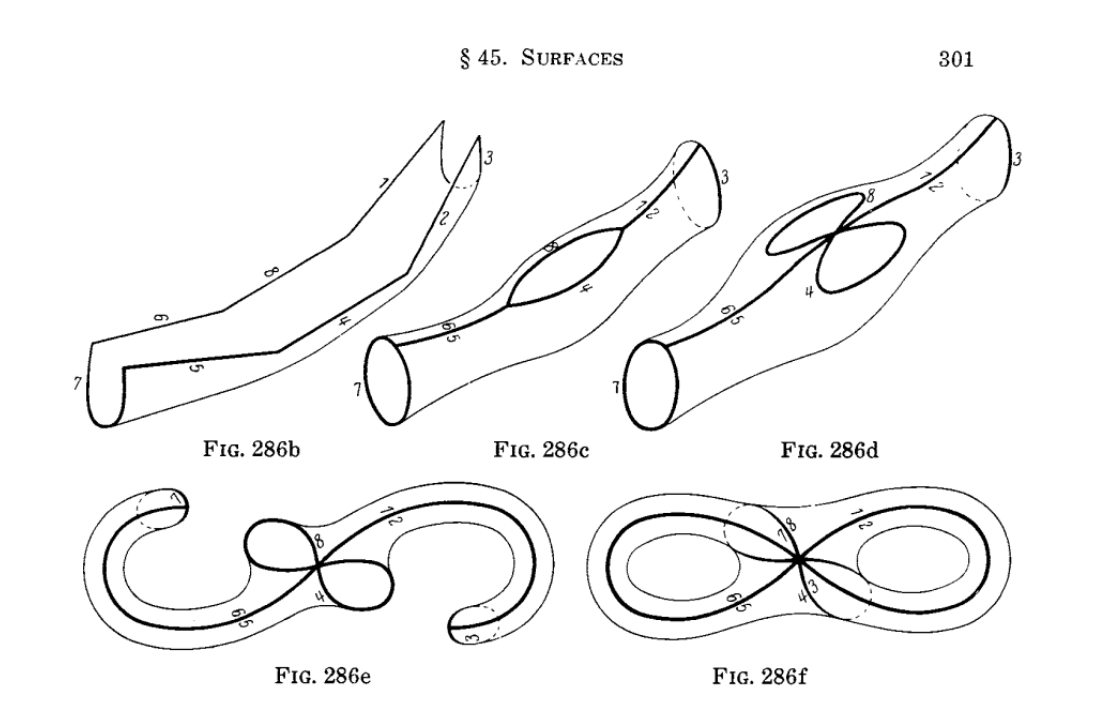
\includegraphics[width=90mm]{two-torus-hilbert.png}
\caption{The geometry of the two torus. Hilbert's \textit{Geometry and the Imagination} \label{overflow}}
\end{figure}

\begin{note}[Abelianization of $\pi_1(M_1)$]
	Consider $\pi_1(M_1) = < a, b ~|~ [a, b]$ as the familiar free group on two
	generators modulo the commutator (where $[a, b] = aba^{-1}b^{-1}$).

	The abelianization of $\pi_1(M_1)$ is then $\pi_1(M_1) \ [\pi_1(M_1), \pi_1(M_1)]$
\end{note}

\subsection{Covering Spaces}

Covering spaces let us (1) calculate fundamental groups of structures and (2)
think about algebraic properties using geometric intuition. (I do not really
understand how yet, so revisit this explanation after some exercise.)

\begin{definition}

	Given some space $X$, the space $\tilde{X}$, along with map $p: \tilde{X} \to
	X$, is a \textbf{covering space} if for each $x \in X$ and any open neighborhood
	$U$ of $x$, $p^{-1}(U)$ is a disjoint union of open sets (called
	\textbf{sheets} in $\tilde{X}$ where each sheet is homeomorphic to $U$.
	
	$p^{-1}(U)$ is allowed to be empty, so $p$ need not be surjective.

\end{definition}

The helicoid (denoted $S$) is a good example that is easy to visualize. The helicoid can be
parameterized as: 

\[x = s \cos 2\pi t \]
\[y = s \sin 2\pi t \]
\[z = t \]

for $s \in (0, \inf), t \in \R$

\begin{figure}[ht!]
\centering
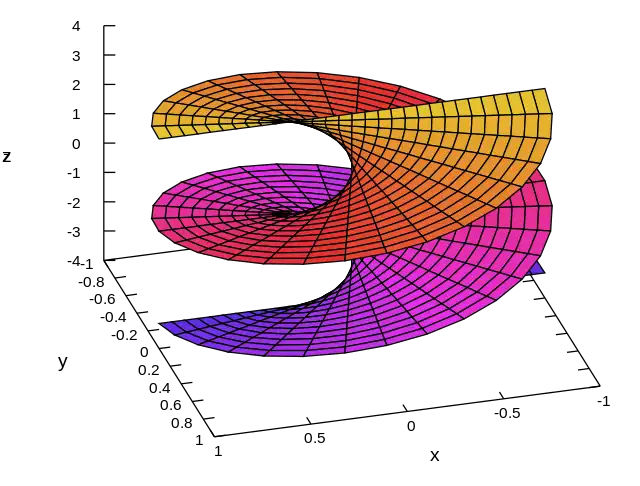
\includegraphics[width=90mm]{./helicoid.png}
\caption{}
\end{figure}

Then $p: S \to \R \setminus \{0\}$ given by $(x, y, z) \mapsto (x, y)$ defines a
covering space.

I found this is best seen by looking at single line segments extending radially
from the origin. Consider $X = (0.5, 1.5) \times \{0\}$. $p^{-1}(X)$ is a
collection of disjoint segments. Our parameterization allows this segment of
the x axis to exist whenever we make one full rotation around the circle. There
are an infinite number of these segments and each maps to $X$ homeomorphically.

\section{Appendix}

\subsection{Presentations}

After more exposure to presentations to describe the group structure of some of
these geometric objects, it became clear that my understanding lacked rigor.

$G = <X~|~R>$ can be considered as the largest possible group with elements
that are words composed of the letters in $X$ \textbf{but} also subject to the
relations described in $R$. "Subject to the relations" means that we can swap
subwords for equivalent subwords or cancel subwords towards reducing different
words to the same underlying group element. 

(For $<a ~|~a^3>$, such reductions look like $aaaaaa = aaa = 1$, $(a^{-1}a^{-1})a = (a)a$)

I have found this hard to reason about the equivalence of words for
presentations (in abstract, not for particular groups) and it turns out that
this problem is very hard. Deciding that words are equivalent in $G$ just from
the generators and relations is unsolvable in general.

\begin{note}
	This problem is called the \textbf{word problem for groups}. In 1911, Max
	Dehn proposed that this problem was an important area of study for group
	theory, whereas prior most mathematicians used normal forms (irreducable
	representations) for group computations which made the word problem less
	relevant.
\end{note}

This does not mean that there do not exist groups where equivalences between
words are obvious. Consider again $<a ~|~a^3>$, any string / word, eg.
$a^4a^{-2}a^3\cdots$, can be reduced monotonically to one of $a, aa, aaa$. 

However, while this idea is intuitive, it is not satisfying, and a more formal
definition of the group describe by a presentation is desired:

\[ G = <X~|~R> = F(X) / <R>^{F(X)} \]

\begin{definition}
	The normal closure of $H$ in $G$ is the smallest normal subgroup containing
	$H$. It is computed by $< \{ xHx^{-1} | x \in G \} >$
\end{definition}

We will prove three properties of the presentation using this formal definition
\href{https://math.stackexchange.com/a/695061/1276086}{motivated by this post}.

\begin{proposition}
	G is generated by the images of $X$ in the quotient group.
\end{proposition}
\begin{proof}
Let $N = <R>^{F(X)}$. Clearly the generating set $\{ xN | x \in X \} \subseteq F(X) / N$. Then the
generated set $< \{ xN | x \in X \} > \subseteq F(X) / N$ as any word
$xNyN \cdots zN$ can be reduced to $(xy \cdots z)N$ and this word is in
$F(X) / N$.

To see the reverse, consider any $gN \in F(X) / N$ and observe $g$ is some word of
elements of $X$. Expand $g$ to the equivalent representation in letters of
$X$, $(xy \cdots z)N$ and see this element lies in the desired generated set.

We finish this proof by constructing an isomorphism by mapping each coset of $<
\{ xN | x \in X \}$ to the coset in that shares its representative $\subseteq
F(X) / N$.
\end{proof}

\begin{proposition}
	G is generated by the images of $X$ in the quotient group.
\end{proposition}

% There is a fundamental result expressing the universal property of 𝐺
% : if 𝐻
%  is any group, and 𝜙:𝑋→𝐻
%  is any map with the property that the images of the elements of 𝑅
%  under 𝜙
%  (you need to say exactly what that means) are all equal to the identity in 𝐻
% , then 𝜙
%  extends uniquely to a group homomorphism 𝐺→𝐻
% . This is not hard to prove from the definition of 𝐺
% .
% You should learn the basic Tietze transformations for manipulating group presentations. Again, the proof that these work can be proved easily from the definition.
% 
% 
% https://math.stackexchange.com/questions/3255411/universal-property-for-presentations

\begin{note}[Free Groups]
	See the \textbf{myasnikov.1.free.groups.pdf} for a category theory flavored exposition on free
	groups, their universal property and role in presentations.
\end{note}

\begin{note}[Universal Property of Free Groups]
Let $S$ be the generating set of a group $F(S)$. For any group $G$ and associated
map $f: S \to G$ (note $f$ is not a homomorphism and is just mapping symbols
into a group), $f$ extends to a unique (homomorphism) $f': F(S) \to G$ that commutes in the following diagram.

\[
\begin{tikzcd}
S \arrow[r, "f"] \arrow[d, "i"'] & G \\
F(S) \arrow[ru, "f'"']           &  
\end{tikzcd}
\]

We proceed with a brief proof and then an example.

If we consider $F(S)$ as reduced words in letters of $S$, let $f' =
f(s_1)\cdots f(s_n)$ and claim this is our extended homomorphism.

Uniqueness can be seen becauase $f'$ must agree with $f$ for each $s \in S$.

\end{note}

Lets construct two isomomorphisms between presentations and groups to understand
what a quotient of this enormous free group and almost just as enormous normal
subgroup actually mean in the context of groups we already understand.

\begin{itemize}
	\item{$\Z \times \Z \cong <a,b~|~[a,b]>$}
	\item{$\S_3 \cong <a,b~|~a^2=b^3=aba^{-1}b^2>$}
\end{itemize}

\begin{proposition}
	$D_3 \cong <x,y~|~x^3=y^2=xyx^{-2}y>$
\end{proposition}

\begin{proof}

	Lets begin by invoking the universal property:
	\[
	\begin{tikzcd}
	{\{x, y\}} \arrow[rd, "f"'] \arrow[r, "i"] & {F(x, y)} \arrow[d, "\phi"] \\
																						 & D_3                        
	\end{tikzcd}
	\]

	Where $F(x, y)$ is our free group on two generator, $i$ is the inclusion map,
	$f$ is a map from our generators to letters in the dihedral group. The
	diagram commutes ($f = \phi i$).

	By definition, our presentation is $F(x, y) / << x^2, y^3, xyx^{-2}y >>$
	(where the $<<->>$ denotes the normal closure). I claim that our universal
	$\theta$ gives us the desired isomorphism when restricted to the quotient
	group.

	Let us expand our commutative diagram by factoring $\phi$ through the
	quotient group:

	\[
	\begin{tikzcd}
	{\{x, y\}} \arrow[rd, "f"'] \arrow[r, "i"] & {F(x, y)} \arrow[d, "\pi"]   \\
																						 & D_3 / N \arrow[d, "\phi'"] \\
																						 & D_3                         
	\end{tikzcd}
	\]

	Where $pi = w \to w << x^2, y^3, xyx^{-2}y >>$ projects words onto
	their cosets and $\phi' = wN \to \phi(w)$. Notice $\phi'$ is well defined as
	the image of every element of the normal closure is the identity ("$\phi$
	respects the relations").

	Then $\phi'$ is surjective as $\phi$ is surjective (every element of $D_3$ is
	word of letters in the image of $f$). To see $\phi'$ is injective, consider
	distinct cosets $aN \neq bN$. Then $\phi'(aN) = \phi'(a)\phi'(N) = \phi'(a) =
	\phi(a)$. Similarly, $\phi'(bN) = \phi(b)$. $\phi(a) \neq \phi(b)$

\end{proof}


\begin{note}
	\textbf{Tietze transforms} define operations on presentations that do not
	change the generated group. Adding and removing both generators and relations
	are allowed if the generator or relation can be derived from other
	information in the presentation.
	$< x, y ~|~ x^2 = y = 1>$
\end{note}

\subsection{Derived Subgroups}

Commutators and derived subgroups appear frequently to describe the structure
of fundamental groups of cell complexes. We will review some definitions and
proofs from elementary algebra.

\begin{definition}
	The \textbf{commutator} of two elements $a, b \in G$ is $a^{-1}b^{-1}ab$ and
	is denoted $[a, b]$.
\end{definition}

\begin{definition}
	$a^x$ is the conjugate of $a$ by $x$ ($xax^{-1}$).
\end{definition}

Clearly the commutator is the identity element if $a$ and $b$ commute in $G$
(hence its name). We derive some pedagogical identities that will be useful.

\begin{definition}
	$[a, b]^x = [a^x,b^x]$
\end{definition}
\begin{proof}
	$xa^{-1}b^{-1}abx^{-1} = xa^{-1}x^{-1}xb^{-1}x^{-1}xax^{-1}xbx^{-1} = [a^x,b^x]$
\end{proof}

\begin{note}
	The set of commutators need not be closed over the group operation.

	Consider the free group on four generators. Then $[a, b][c, d] =
	a^{-1}b^{-1}abc^{-1}d^{-1}cd$. This is not a commutator in this group (there
	are no two elements $x, y$ such that $[x, y] = [a, b][c, d]$.
\end{note}

Even though products of commutators are not themselves commutators in general,
the subgroup \textit{generated} by all commutators in a group is certainly closed over
the group operation. This leads naturally to the derived subgroup.

\begin{definition}
	The group generated by all of the commutators in $G$ is the \textbf{derived
	subgroup} of $G$, denoted $[G, G]$ or $G'$.
\end{definition}

\begin{theorem}
	$[G, G] \trianglelefteq G$
\end{theorem}

\begin{proof}
	$([a, b] \cdots [e, f])^x = ([a^x, b^x] \cdots [e^x, f^x])$
\end{proof}

\begin{theorem}
	If the quotient group $G / N$ is abelian, then $[G, G] \subseteq N$. In other
	words, the derived subgroup the smallest subgroup that abelianizes $G$.
\end{theorem}

\begin{proof}
	Let $N$ be some normal subgroup of $G$, then $N$ abelianizes $G$ iff for each
	$x, y \in G$, $xyN = yxN$. Then $N = y^{-1}x^{-1}yxN$ (the group operation is
	well-defined as $N$ is normal) so $y^{-1}x^{-1}yx \in N$. 

	Certainly the set of commutators must be included in $N$. So any minimal $N$
	is the minimal group generated by these commutators. But this is exactly $[G,
	G]$.
\end{proof}

\begin{definition}
	$G / [G, G]$ is the abelianization of $G$ and sometimes denoted $G^{ab}$.
\end{definition}

\end{document}
